\graphicspath{{Figs/montecarlo/}}

%
% To start the document, use
%  \chapter{...}
% For lover level, sections use
%  \section{...}
%  \subsection{...}
%
\chapter{Reversed Monte Carlo Scattering: ARTS-MC}
 \label{sec:montecarlo}


%
% Document history, format:
%  \starthistory
 %    date1 & text .... \\
%    date2 & text .... \\
%    ....
%  \stophistory
%
\starthistory
  120410 & Moved from user guide to theory document.\\
  300504 & Created and written by Cory Davis.\\
\stophistory


%
% Symbol table, format:
%  \startsymbols
%    ... & \verb|...| & text ... \\
%    ... & \verb|...| & text ... \\
%    ....
%  \stopsymbols
%
%

%
% Introduction
%




\section{Introduction}
 \label{sec:montecarlo:intro}

%%%%%%%%%%%%%%%%%%%%%%%%%%%%%%%%%%%%%%%%%%%%%%%%%%%%%%%%%% 
\section{Model[FIXME: needs updating to MCGeneral]}
 \label{sec:montecarlo:model}
The radiative transfer model solves the vector
radiative transfer equation (VRTE):
\begin{eqnarray}
\frac{d\mathbf{I(n)}}{ds}=-\mathbf{K(n)I(n)} +
\mathbf{K_a(n)}I_b(T) +\nonumber\\
\int_{4\pi}\mathbf{Z(n,n')I(n')}d\mathbf{n'}
\label{vrte}
\end{eqnarray}
where $\mathbf{I}$ is the 4 element column vector of radiances
$\mathbf{I}=\left[I,Q,U,V\right]^T$ with units
(Wm$^{-2}\mu$m$^{-1}$sr$^{-1}$). This will be referred to as the
Stokes vector, although normally the Stokes vector is expressed in
units of intensity.  $s$ is distance along direction $\mathbf{n}$ and
$I_b$ is the Planck radiance. $\mathbf{K(n)}$, $\mathbf{K_a(n)}$,
and $\mathbf{Z(n,n')}$ are the bulk extinction matrix, absorption
coefficient vector and phase matrix of the medium respectively.  For
 brevity these have been expressed as bulk optical
properties, where individual single scattering properties have been
multiplied by particle number density and averaged over all
orientations and particle types. The argument $\mathbf{n}$ has been
retained to signify that in general these properties depend on the
direction of propagation. 

To apply Monte Carlo integration to the problem, the VRTE needs to be expressed in integral form. (e.g. \cite{hochstadt:64})
\begin{eqnarray}
\lefteqn{\mathbf{I(n,s_0)}=\mathbf{O(u_0,s_0)I(n,u_0)}+}\nonumber\\
& \int_{u_0}^{s_0}\mathbf{O(s',s_0)}\left(\mathbf{K_a(n)}I_b(T) +\int_{4\pi}\mathbf{Z(n,n')}\mathbf{I(n')}d\mathbf{n'}\right)ds'\nonumber
\end{eqnarray}
\begin{equation}
\label{intVRTE}
\end{equation}
, where $\mathbf{O(s',s)}$ is the evolution operator defined by
\cite{landi:85}. $\mathbf{u_0}$ is the point where the line of sight intersects
the far boundary of the scattering domain, and $\mathbf{s_0}$ is the
exit point where the outgoing Stokes vector is calculated.

If we consider a scalar antenna response function,
$\psi=\psi(\theta,\phi)=\psi(\mathbf{n})$, where $\psi(\mathbf{n})$ is
normalised such that $\int_{4\pi}\psi(\mathbf{n})dn=1$, then the
observed Stokes vector will $\mathbf{I_{ant.}(n,s_0)}$ will be

\begin{equation}
\mathbf{I_{ant.}(n,s_0)}=\int_{4\pi}\psi(\mathbf{n'})\mathbf{I(n',s_0)}d\mathbf{n'}
\label{antInt}
\end{equation}

If we apply Monte Carlo integration with importance samping to
Eq. \ref{antInt} and sample $\mathbf{n'}$ according to a probability
density function (PDF) equal to $\psi(\mathbf{n'})$ then an unbiased
estimate of Eq. \ref{antInt} is given by (e.g. \cite{press:1992:numerical})

\begin{eqnarray}
\mathbf{I_{ant.}(n,s_0)}&=&\int_{4\pi}\mathbf{I(n',s_0)}\psi(\mathbf{n'})d\mathbf{n'}\\
&=&\langle \mathbf{I(n',s_0)} \rangle_\psi
\label{antIntMC}
\end{eqnarray}

We now require a Monte Carlo estimate of the integrand in
Eq. \ref{antIntMC}, which is given by Eq. \ref{intVRTE}.  First, we
re-express \ref{intVRTE} as a single integral, for simplicity dropping
the prime on $\mathbf{n'}$,

\begin{equation}
\mathbf{I(n,s_0)}=\int^{s_0}_\infty\left\{\begin{array}{rl}
\mathbf{O(s',s_0)}\left(\mathbf{K_a(n)}I_b(T)
+\int_{4\pi}\mathbf{Z(n,n')}\mathbf{I(n')}d\mathbf{n'}\right) & s'< s'_{boundary} \\
\frac{\mathbf{O(u_0,s_0)I(n,u_0)}g}{\int^\infty_{u_0}gds} & s'\ge s'_{boundary}
\end{array}ds'\right.
\label{inorouteq}
\end{equation}
, where $g$ is the PDF we will eventually use to sample pathlength,
$\Delta s$. $s'_{boundary}$ represents the pathlength corresponding to
the boundary of the domain opposite the line of sight.
The integrand Eq. \ref{inorouteq} is a piecewise function of the
path distance, where path distances corresponding to positions outside
the modelled domain give a boundary radiance attenuated by evolution
operator over the length of the path within the model domain, and path
distances corresponding to points within the modelled atmosphere give
a sum of emission and scattering attenuated by the evolution operator
over the distance between the point and the atmosphere exit. 
The reader
could easily verify that evaluating Eq. \ref{inorouteq} gives
Eq. \ref{intVRTE}. 

The aim in importance sampling is to choose probability density functions
(PDFs) for the independent variables that are
as close as possible to being proportional to the integrand
\cite{liu:01}. This concentrates computational effort on regions where
the integrand is most significant and also reduces the variance in the contributions of each photon, thus reducing
the number of photons and hence CPU time required to give a
prescribed accuracy.  Eq. \ref{intVRTE} suggests that the PDF for
sampling path length, where path length is the distance traced backwards
from the sensor, $\Delta s=\left|\mathbf{s}-\mathbf{s'}\right|$, should be proportional in some way to the evolution
operator $\mathbf{O(s',s)}$. 

In general there is no closed form expression for $\mathbf{O(s',s)}$.
However, in cases where the extinction matrix is constant along a
propagation path
\begin{equation}
\mathbf{O(s',s)}=\exp\left(-\mathbf{K}\Delta s\right)
\label{OconstK}
\end{equation}
In ARTS a propagation path consists of a set of coordinates
indicating where the path intersects with grid surfaces.  If the
extinction matrix in the path segment between two such points is
considered constant, $\mathbf{K}=(\mathbf{K_j}+\mathbf{K_{j+1}})/2$,
the evolution operator between two arbitrary points $\mathbf{s_0}$ and
$\mathbf{s}_N$ is
\begin{eqnarray}
\mathbf{O}(\mathbf{s}_0,\mathbf{s}_N) =
\mathbf{O}(\mathbf{s}_{N-1},\mathbf{s}_N)
\mathbf{O}(\mathbf{s}_{N-2},\mathbf{s}_{N-1}) \dots \nonumber\\
\mathbf{O}(\mathbf{s}_1,\mathbf{s}_2)\mathbf{O}(\mathbf{s}_0,\mathbf{s}_1),
\end{eqnarray}
, where $\mathbf{O(s_i,s_{i+1})}$ is given by Eq. \ref{OconstK}.

Since PDFs are scalar functions, and that we consider the first element of the
Stokes vector most important, we choose the pathlength PDF to be proportional to the
(1,1) element of $\mathbf{O(s',s)}$,

\begin{equation}
g(\Delta s)=\tilde{k}\tilde{O_{11}}(\Delta s)
\label{gDeltas}
\end{equation}
This is sampled by taking a random number and solving 
\begin{equation}
\tilde{O_{11}}(\Delta s)=r.
\label{solvefor0}
\end{equation}
for $\Delta s$.  Here, 
\begin{equation}
\tilde{k}=\frac{1}{\left(\Delta s_B-\Delta s_A\right)}
\ln\left(\frac{O_{11}^A}{O_{11}^B}\right)
\end{equation}
, which, for cases where the extinction matrix is diagonal, is equal to $K_{11}=(K_{11}^A+K_{11}^B)/2$.

With pathlength sampled according to Eq. \ref{solvefor0}, the Monte
Carlo estimate for Eq. \ref{inorouteq} becomes
\begin{eqnarray}
\mathbf{I(n,s_0)}&=&\int^{s_0}_\infty\left\{\begin{array}{rl}
\frac{\mathbf{O(s',s_0)}}{g(\Delta s)}\left(\mathbf{K_a(n)}I_b(T)
+\int_{4\pi}\mathbf{Z(n,n')}\mathbf{I(n')}d\mathbf{n'}\right) & s'< s'_{boundary} \\
\frac{\mathbf{O(u_0,s_0)I(n,u_0)}}{1-\tilde{O_{11}}(\Delta s)} & s'\ge s'_{boundary}
\end{array}g(\Delta s)ds'\right.\\
&\approx&\left\langle\left\{\begin{array}{rl}
\frac{\mathbf{O(s',s_0)}}{g(\Delta s)}\left(\mathbf{K_a(n)}I_b(T)
+\int_{4\pi}\mathbf{Z(n,n')}\mathbf{I(n')}d\mathbf{n'}\right) & s'< s'_{boundary} \\
\frac{\mathbf{O(u_0,s_0)I(n,u_0)}}{1-\tilde{O_{11}}(\Delta s)} & s'\ge s'_{boundary}
\end{array}\right.\right\rangle
\end{eqnarray} 

Likewise, new incident directions
($\theta_{inc},\phi_{inc}$) should be sampled from a PDF proportional
to
$\mathbf{Z}(\theta_{scat},\phi_{scat},\theta_{inc},\phi_{inc})$.

%%%%%%%%%%%%%%%%%%%%%%%%%%%%%%%%%%%%%%%%%%%%%%%%%%%%%%%%%%%%%
\subsection{Algorithm [FIXME:Needs updating to MCGeneral]}
 \label{sec:montecarlo:alg}
The model algorithm proceeds as follows:

\begin{enumerate}
\item
Begin at the cloud box exit point with a new photon. Sample a
  path length, $\Delta s$ along the first line of sight using the PDF
\begin{equation}
g_0(\Delta s)=\frac{\tilde{k}\tilde{O_{11}}(\Delta s)}
{1-O_{11}(\mathbf{u_0,s_0})}.
\label{g0Deltas}
\end{equation}
, where $\tilde{O_{11}}(\Delta s)$, is the piecewise exponential
function that includes $O_{11}(\mathbf{s',s})$ values at points
where the line of sight intersects with grid surfaces.
Between two such adjacent intersections, $A$ and $B$, the function
$\tilde{O_{11}}(\Delta s)$ is given by
\begin{equation}
\tilde{O_{11}}(\Delta s)=O_{11}(\Delta s_A)\exp\left(-\tilde{k}\left(\Delta s-\Delta
s_A\right)\right)
\label{O11}
\end{equation}
, and
\begin{equation}
\tilde{k}=\frac{1}{\left(\Delta s_B-\Delta s_A\right)}
\ln\left(\frac{O_{11}^A}{O_{11}^B}\right)
\end{equation}
, which, for cases where the extinction matrix is diagonal, is equal to $K_{11}=(K_{11}^A+K_{11}^B)/2$.
The denominator in Eq. \ref{g0Deltas} ensures an emission or scattering
event for each photon in the initial line of sight.
Eq. \ref{g0Deltas} is sampled by taking a random number (from the
uniform distribution [0,1]), $r$, and solving 
\begin{equation}
\frac{1-\tilde{O_{11}}(\Delta s)}{1-O_{11}(\mathbf{u_0,s_0})}=r.
%\label{solvefor0}
\end{equation}
for $\Delta s$.
%%%%%%%%%%%%%%%%%%%%%%%%%%%%%%%%%%%%%%%%%%%%%%%%%%%%%%%%%%%%%%%%
\item
Another random number, $r$, is drawn to choose between emission and scattering.  We first define an albedo-like quantity
\begin{equation}
\tilde{\omega}=1-\frac{K_{a1}(\mathbf{n_{0},s_{1}})}{K_{11}(\mathbf{n_{0},s_{1}})}
\end{equation}
Note: we can't use the actual single-scattering albedo as this depends
on the polarization state of the incident radiation.  If $r>\tilde{\omega}$, then the event is considered to be emission,
the reversed ray tracing is terminated, and the Stokes vector
contribution of the $i$th photon is
\begin{equation}
\mathbf{I^i(n,s_0)}=\frac{\mathbf{O(s_1,s_0)}\mathbf{K_a(n_0,s_1)}
  I_b(T,\mathbf{s_i})}{g_0(\Delta s) \left(1-\tilde{\omega}\right)}
\label{Iemission2}
\end{equation}
, where the index $i$ signifies photon number. Return to step 1.

Otherwise, if $r\le\tilde{\omega}$
we have a scattering event.
%3%%%%%%%%%%%%%%%%%%%%%%%%%%%%%%%%%%%%%%%%%%%%%%%
\item
At the scattering point sample a new incident direction
  $(\theta_{inc},\phi_{inc})$ according to 
\begin{equation}
g(\theta_{inc},\phi_{inc})=\frac{Z_{11}(\theta_{scat},\phi_{scat},
\theta_{inc},\phi_{inc})\sin(\theta_{inc})}{K_{11}(\theta_{scat},\phi_{scat})
  - K_{a1}(\theta_{scat},\phi_{scat})}
\label{gdir}
\end{equation}
, which is
sampled by the rejection method as described in \cite{liu:01}.

Calculate the matrix
\begin{equation}
\mathbf{Q_k}=\mathbf{Q_{k-1}q_k}
\label{Q}
\end{equation}
, where
\begin{equation}
\mathbf{q_k}=\frac{\sin(\theta_{inc})_k
  \mathbf{O(s_k,s_{k-1})}\mathbf{Z(n_{k-1},n_k)}}
  {g\left(\Delta s\right)g(\theta_{inc},\phi_{inc}) \tilde{\omega}} ,
\label{q}
\end{equation}
and $\mathbf{Q_0}={1}$. The index $k$ represents the
scattering order.
%4%%%%%%%%%%%%%%%%%%%%%%%%%%%%%%%%%%%%%%%%%%%%%%%%%%
\item
Choose a path length along the new direction according to
If $r<O_{11}(\mathbf{u_{k},s_k})$, where $\mathbf{u}_{k}$ is the
  boundary of the scattering domain in the current line of sight, the
  photon leaves the scattering domain, and the contribution for photon $i$ is
\begin{equation}
\mathbf{I^i(n,s_0)}=\frac{\mathbf{Q_k}\mathbf{O(u_k,s_k)I(n_k,u_k)}}{O_{11}(\mathbf{u_{k},s_k})}
\label{Ikmax2_1}
\end{equation}
, where 
$\mathbf{I(n_k,u_k)}$ is the incoming radiance at $\mathbf{u}_{k}$.  This is calculated with the standard ARTS clear-sky
routine. Return to step 1.

Otherwise, if the sampled path length keeps the path within the
scattering domain...
%%%%%%%%%%%%%%%%%%%%%%%%%%%%%%%%%%%%%%%%%%%%%%%%%%%%%
\item
As in step 2, calculate 
$\tilde{\omega}$ at the new point, $\mathbf{s_{k+1}}$, and draw a uniform
  random deviate, $r$.

If $r>\tilde{\omega}$, then the event is considered to be emission,
the reversed ray tracing is terminated, the Stokes vector contribution is
\begin{equation}
\mathbf{I^i(n,s_0)}=\frac{\mathbf{Q_k O(s_{k+1},s_k)}
  \mathbf{K_a(n_k,s_{k+1})} I_b(T,\mathbf{s_{k+1}})}
  {g\left(\Delta s\right)\left(1-\tilde{\omega}\right)}
\label{Iemission3}
\end{equation}
, and we return to step 1.

Otherwise, if $r\le\tilde{\omega}$
we have a scattering event and we return to step 3.
\item
Once the prescribed number, $N$,  of photon contributions,
$\mathbf{I^i(n,s_0)}$, have been calculated, the cloud box exit Stokes
vector is given by
\begin{equation}
\mathbf{I(n,s_0)}=\mathbf{O(u_0,s_0)I(n,u_0)}+\langle\mathbf{I^i(n,s_0)}\rangle.
\label{cbexit}
\end{equation}
, with an estimated error for each Stokes index, $j$,  of
\begin{equation}
\delta I_j=\sqrt{\frac{\langle I_j^2\rangle-\langle I_j\rangle^2}{N}}.
\label{error}
\end{equation}
\end{enumerate}
When simulating an MLS measurement, an extra clear sky RT calculation
is performed from the cloud box exit to the sensor, with the Monte
Carlo result from Eq. \ref{cbexit} taken as the radiative background.

\begin{figure}[!ht]
\begin{center}
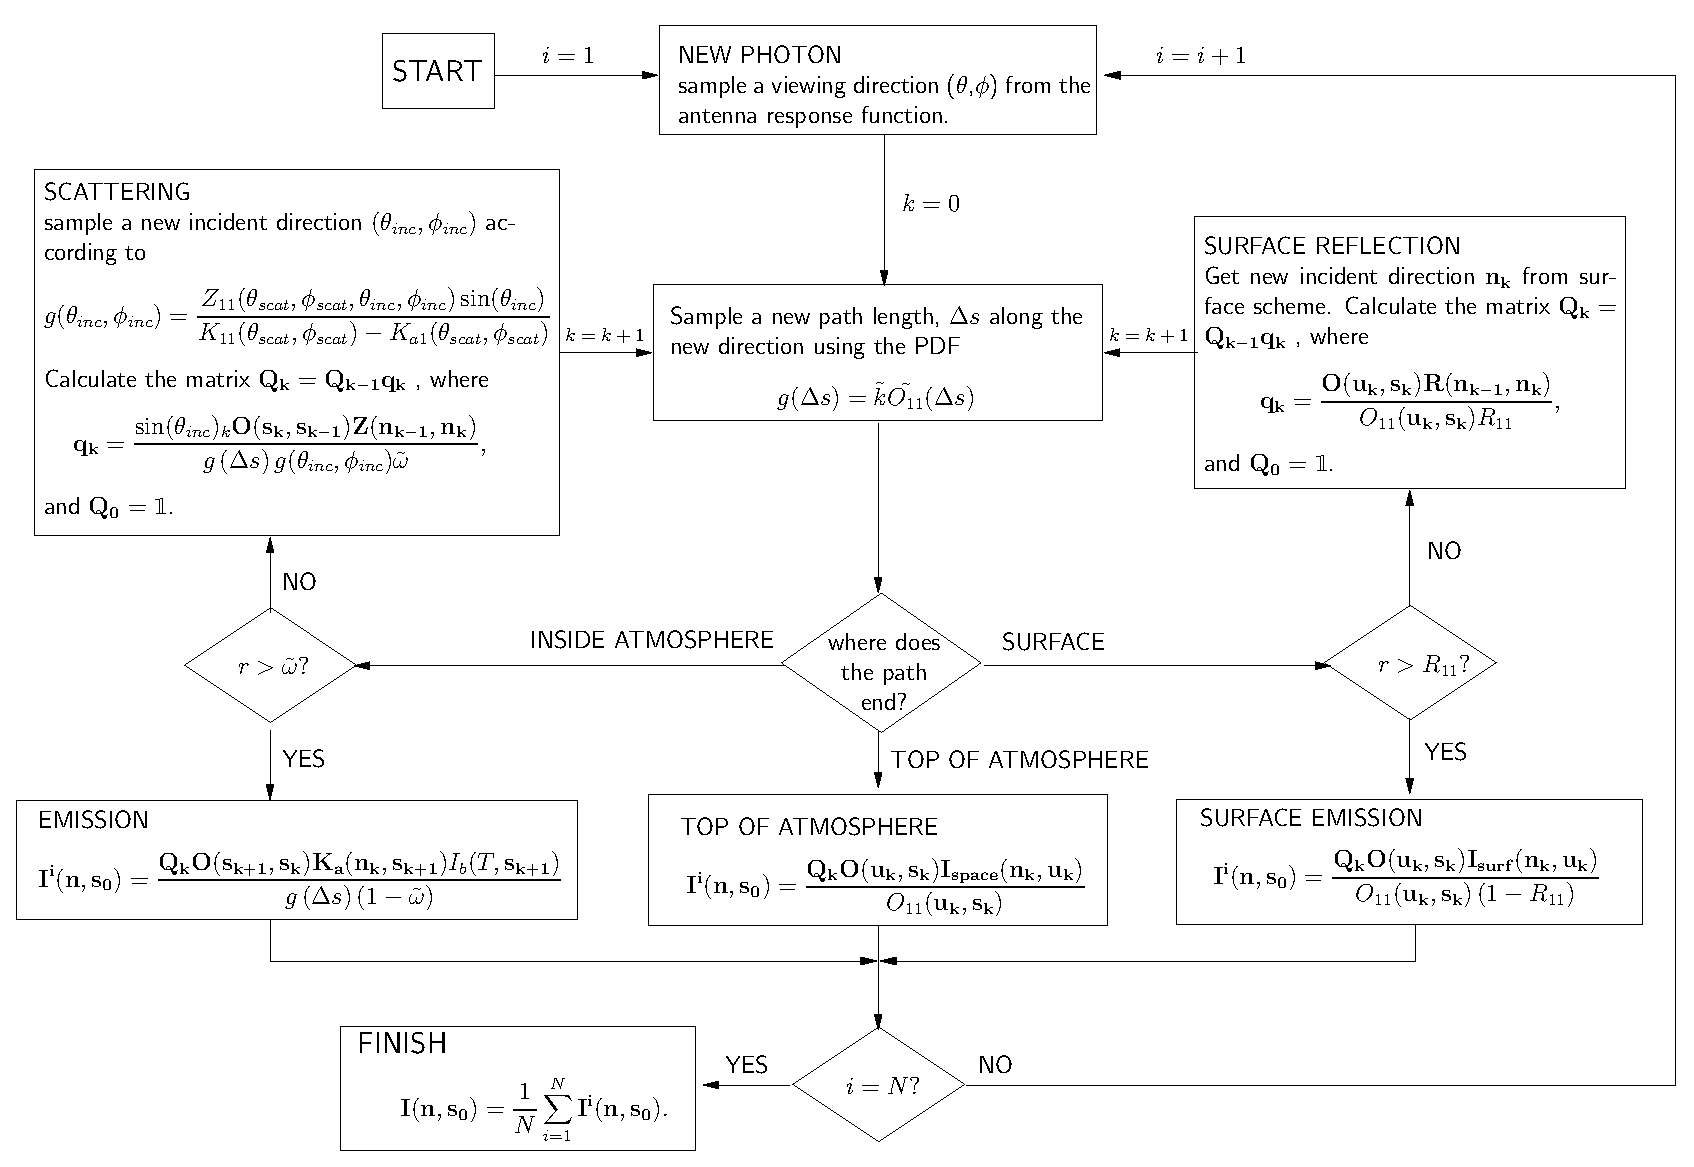
\includegraphics[width=\vsize,angle=90]{flowchart2}
\caption{Flowchart illustrating MCGeneral algorithm}
\end{center}
\label{fig:montecarlo:flowchart}
\end{figure}

 
%%% Local Variables: 
%%% mode: latex 
%%% TeX-master: "uguide" 
%%% End:

